\chapter{THỰC NGHIỆM VÀ ĐÁNH GIÁ}
\ifpdf
    \graphicspath{{Chapter4/Chapter4Figs/PNG/}{Chapter4/Chapter4Figs/PDF/}{Chapter4/Chapter4Figs/}}
\else
    \graphicspath{{Chapter4/Chapter4Figs/EPS/}{Chapter4/Chapter4Figs/}}
\fi

\section{Mở đầu}
Mục đích của chương này là trình bày một số kết quả thực nghiệm trên bộ dữ liệu thu thập được. Qua đó đánh giá, nhận định và so sánh các thuật toán gom cụm, cũng như xem xét sự ảnh hưởng của các thông số đến kết quả, thời gian thực thi các thuật toán.

\section{Tổng quan về bộ dữ liệu}
Bộ dữ liệu gồm các bài viết từ Twitter. Dữ liệu được lấy thông qua 2 luồng khác nhau: Twitter Search API và Twitter Streaming API. Một danh sách 115 từ khóa được sử dụng để chọn lọc những bài viết đề cập đến sự kiện nào đó, thay vì chỉ là những bài đăng cá nhân. Các từ khóa được chia theo 14 chủ đề, dựa trên 13 chủ đề ban đầu của tài liệu hướng dẫn gán nhãn TDT 2004 \cite{TDT2004Annotation}. %liên quan đến các sự kiện thường được đăng tin.

Mỗi tweet trong tập dữ liệu bao gồm các thông tin sau: ID tweet do Twitter tạo, ID người dùng đăng tweet, tên tài khoản người đăng tweet, nội dung tweet, thời gian đăng tweet, thời gian tweet được thu thập vào hệ thống.

Bộ dữ liệu thử nghiệm thứ nhất gồm 9,211 tweets tiếng Việt, được thu thập thông qua Search API trong khoảng thời gian 11 ngày, từ 31/1/2017 đến 10/2/2017.

%Bộ dữ liệu thử nghiệm thứ hai gồm 57,915 tweets tiếng Việt, được thu thập thông qua Streaming API trong khoảng thời gian 25 ngày, từ 18/5/2017 đến 10/6/2017.

	\begin{table}[H]
%		\centering
		\setlength\extrarowheight{3pt}
		\begin{tabular}{|p{4cm}|p{10cm}|}
			\hline
			Accident      & tai nạn, chết người, thảm khốc, rơi máy bay, tai nạn máy bay, máy bay mất tích, \#tainan, \#tainạn, \#chetnguoi, \#chếtngười \\
			\hline
			Act of War or Violence, Military News & thả bom, đánh bom, tên lửa, hạt nhân, bom hạt nhân, đầu đạn hạt nhân, vũ khí, vũ khí huỷ diệt, xả súng, khủng bố, \#đánhbom, \#khủngbố \\
			\hline
			Bizarre News and World Records & kỷ lục thế giới, Guinness, chuyện lạ có thật, chuyện lạ khó tin, chuyện lạ bốn phương, phong tục kỳ lạ \\
			\hline
			Celebrity and Human Interest News & tổng thống, tổng bí thư, thủ tướng, chủ tịch nước, phát ngôn, phát ngôn gây sốc, Barack Obama, Donald Trump, Putin, Shinzo Abe, Tập Cận Bình, Rodrigo Duterte, Nguyễn Phú Trọng, Nguyễn Xuân Phúc, Trần Đại Quang, Ca sĩ, Hoa hậu, Người mẫu,	Diễn viên \\
			\hline
			Election      & đại hội đảng, bầu cử, bầu cử đại biểu quốc hội, bầu cử tổng thống, \#baucu, \#bầucử \\
			\hline
			Financial     & xăng lên giá, xăng giảm giá, chứng khoán, bất động sản, chấn động thị trường, \#taichinh, \#tàichính \\
			\hline
			General       & tin nóng, tin giật gân, \#tinnong, \#tinnóng, \#tingiatgan, \#tingiậtgân \\
			\hline
			Legal and Criminal Case & cướp, giết người, khủng khiếp, hãm hiếp, hiếp dâm, lạm dụng tình dục, tham ô, tham nhũng, \#gietnguoi, \#giếtngười \\
			\hline
			Natural Disaster & động đất, sóng thần, lũ lụt, mưa đá, thiên tai, bão lớn, \#thientai, \#thiêntai \\
			\hline
			New Law       & dự thảo luật, điều luật mới, chính sách mới \\
			\hline
			Political Meeting and Statement & tổng thống, tổng bí thư, thủ tướng, chủ tịch nước, hội nghị, cuộc gặp gỡ, gặp mặt, họp mặt \\
			\hline
			Scandal and Hearing & bê bối, quấy rối, quấy rối tình dục, hầu tòa, ra tòa, scandal, \#scandal \\
			\hline
			Science and Discovery & phát minh, giải nobel, giải fields, khám phá mới, phát hiện mới \\
			\hline
			Sport         & đội tuyển bóng đá quốc gia, đội tuyển U19, U19 Hoàng Anh Gia Lai, SeaGames, AFC Suzuki Cup, \#bongda, \#bóngđá \\
			\hline
		\end{tabular}%
		\caption{Danh sách từ khóa để thu thập dữ liệu}
		\label{tab:twitterkeywords}%
	\end{table}%

Bộ dữ liệu có thể được tải về từ địa chỉ: \url{https://drive.google.com/open?id=0B6FWPU7hs7CIRUZudGl3bG9DbEk}

\section{Thiết lập thực nghiệm, cách đánh giá}
Sử dụng 4 thuật toán: Gom cụm theo k-Nearest Neighbor, gom cụm với boost cho Named Entity, gom cụm dùng LSH và LSH cải tiến. 

Ta đánh giá và so sánh kết quả về thời gian xử lý và chất lượng cụm thông qua một số độ đo đã trình bày ở mục \ref{clusterEvalMetrics}: intracluster distance, intercluster distance.

Cả 4 thuật toán đều sử dụng giá trị ngưỡng để xét điểm dữ liệu có thuộc cụm hay không. Thuật toán Nearest Neighbor và Boost Named Entity sử dụng ngưỡng về \textit{độ tương đồng} MergeThreshold, ngược lại thuật toán LSH sử dụng ngưỡng \textit{khoảng cách} NoveltyThreshold. Thực chất $NoveltyThreshold = 1 - MergeThreshold$ nên ta vẫn có thể quy đổi giá trị giữa chúng để so sánh kết quả các thuật toán. Tất cả giá trị ngưỡng trong chương này sẽ được quy đổi về giá trị của \textbf{MergeThreshold} tương ứng.

Riêng thuật toán LSH có thêm các thông số như: số hashtable, số siêu phẳng, lượng document tối đa cho mỗi bucket,... ta sẽ cần xét sự ảnh hưởng của chúng đến quá trình và kết quả gom cụm.
\section{Kết quả thực nghiệm}

	\subsection{Thay đổi MergeThreshold}
	Dưới đây là kết quả các thuật toán khi thay đổi giá trị MergeThreshold từ 0.1 đến 0.9:
		\begin{table}[H]
			\centering
			\setlength\extrarowheight{3pt}
			\begin{tabular}{|l|p{1.4cm}|p{1.5cm}|p{2cm}|p{2cm}|p{1.8cm}|}
				\hline
				Thuật toán  & Số cụm   & Entropy & Intracluster distance & Intercluster distance & Thời gian (ms) \\
				\hline
				KNN   & 100   & 3.453057 & 0.483357 & 0.996435 & 279,439 \\
				\hline
				Boost Named Entity & 134 & 4.507409	& 0.847914 & 1	& 3,462,536 \\
				\hline
				LSH   & 510   & 2.609871 & 0.255654 & 0.996635 & 30,704 \\
				\hline
				LSH+  & 510   & 2.609871 & 0.255654 & 0.996635 & 29,687 \\
				\hline
			\end{tabular}%
		
			\caption{MergeThreshold = 0.1} \label{tab:table_4_1}%
		\end{table}
		
		\begin{table}[H]
%			\centering
			\setlength\extrarowheight{3pt}
			\begin{tabular}{|l|p{1.4cm}|p{1.5cm}|p{2cm}|p{2cm}|p{1.8cm}|}
				\hline
				Thuật toán  & Số cụm   & Entropy & Intracluster distance & Intercluster distance & Thời gian (ms) \\
				\hline
				KNN   & 1358  & 2.640104 & 0.239420 & 0.995582 & 239,357 \\
				\hline
				Boost Named Entity & 134 & 4.507409 & 0.847914 & 1 & 3,157,517 \\
				\hline
				LSH   & 2545  & 2.431249 & 0.150437 & 0.994624 & 30,274 \\
				\hline
				LSH+  & 2510  & 2.434242 & 0.151118 & 0.994679 & 30,629 \\
				\hline
			\end{tabular}%
			\caption{MergeThreshold = 0.2} \label{tab:table_4_2}%
		\end{table}
		
		\begin{table}[H]
			\centering
			\setlength\extrarowheight{3pt}
			\begin{tabular}{|l|p{1.4cm}|p{1.5cm}|p{2cm}|p{2cm}|p{1.8cm}|}
				\hline
				Thuật toán  & Số cụm   & Entropy & Intracluster distance & Intercluster distance & Thời gian (ms) \\
				\hline
				KNN   & 3097  & 2.418943 & 0.128281 & 0.993779 & 242,266 \\
				\hline
				Boost Named Entity & 135  & 4.523543 & 0.844617 & 0.999963 & 4,240,763 \\
				\hline
				LSH   & 3955  & 2.340955 & 0.091359 & 0.992901 & 29,495 \\
				\hline
				LSH+  & 3925  & 2.342387 & 0.092103 & 0.992924 & 30,394 \\
				\hline		
			\end{tabular}%
			\caption{MergeThreshold = 0.3} \label{tab:table_4_3}%
		\end{table}
		
		\begin{table}[H]
			\centering
			\setlength\extrarowheight{3pt}
			\begin{tabular}{|l|p{1.4cm}|p{1.5cm}|p{2cm}|p{2cm}|p{1.8cm}|}
				\hline
				Thuật toán  & Số cụm   & Entropy & Intracluster distance & Intercluster distance & Thời gian (ms) \\
				\hline
				KNN   & 4184  & 2.341865 & 0.079299 & 0.992050 & 241,671 \\
				\hline
				Boost Named Entity & 143 & 4.65682 & 0.845813 & 0.999771 & 6,031,529 \\
				\hline
				LSH   & 4734  & 2.309055 & 0.062843 & 0.991542 & 32,644 \\
				\hline
				LSH+  & 4710  & 2.309963 & 0.063133 & 0.991563 & 32,858 \\
				\hline
			\end{tabular}%
			\caption{MergeThreshold = 0.4} \label{tab:table_4_4}%
		\end{table}
		
		\begin{table}[H]
			\centering
			\setlength\extrarowheight{3pt}
			\begin{tabular}{|l|p{1.4cm}|p{1.5cm}|p{2cm}|p{2cm}|p{1.8cm}|}
				\hline
				Thuật toán  & Số cụm   & Entropy & Intracluster distance & Intercluster distance & Thời gian (ms) \\
				 \hline
				KNN & 4778 & 2.308508 & 0.051345 & 0.991100 & 270,376  \\
				\hline
				Boost Named Entity & 164 & 4.330696 & 0.832134 & 0.999370 & 8,562,791 \\
				\hline
				LSH & 5171 & 2.290040 & 0.043537 & 0.990804 & 29,906  \\
				\hline
				LSH+ & 5155 & 2.290858 & 0.043968 & 0.990812 & 31,688  \\
				\hline
			\end{tabular}%
			\caption{MergeThreshold = 0.5} \label{tab:table_4_5}%
		\end{table}
		
		\begin{table}[H]
			\centering
			\setlength\extrarowheight{3pt}
			\begin{tabular}{|l|p{1.4cm}|p{1.5cm}|p{2cm}|p{2cm}|p{1.8cm}|}
				\hline
				Thuật toán  & Số cụm   & Entropy & Intracluster distance & Intercluster distance & Thời gian (ms) \\
				\hline
				KNN & 5153 & 2.291737 & 0.034421 & 0.990652 & 269,129  \\
				\hline
				Boost Named Entity & 192 & 4.195825 & 0.820760 & 0.999014 & 10,740,287\\
				\hline
				LSH & 5468 & 2.279607 & 0.030737 & 0.990459 & 29,418  \\
				\hline
				LSH+ & 5455 & 2.280260 & 0.031068 & 0.990461 & 34,689  \\
				\hline
			\end{tabular}%
			\caption{MergeThreshold = 0.6} \label{tab:table_4_6}%
		\end{table}
		
		\begin{table}[H]
			\centering
			\setlength\extrarowheight{3pt}
			\begin{tabular}{|l|p{1.4cm}|p{1.5cm}|p{2cm}|p{2cm}|p{1.8cm}|}
				\hline
				Thuật toán  & Số cụm   & Entropy & Intracluster distance & Intercluster distance & Thời gian (ms) \\
			    \hline
				KNN & 5499 & 2.281347 & 0.022001 & 0.990179 & 255,027  \\
				\hline
				Boost Named Entity & 232 & 4.042305 & 0.775990 & 0.998580 & 14,239,743\\
				\hline
				LSH & 5759 & 2.271498 & 0.020295 & 0.990157 & 30,494  \\
				\hline
				LSH+ & 5751 & 2.271919 & 0.020370 & 0.990165 & 32,434  \\
				\hline
			\end{tabular}%
			\caption{MergeThreshold = 0.7} \label{tab:table_4_7}%
		\end{table}
		
		\begin{table}[H]
			\centering
			\setlength\extrarowheight{3pt}
			\begin{tabular}{|l|p{1.4cm}|p{1.5cm}|p{2cm}|p{2cm}|p{1.8cm}|}
				\hline
				Thuật toán  & Số cụm   & Entropy & Intracluster distance & Intercluster distance & Thời gian (ms) \\
			     \hline
				KNN & 5884 & 2.269258 & 0.010429 & 0.989852 & 260,766  \\
				\hline
				Boost Named Entity & 291 & 3.844293 & 0.750010 & 0.998067 & 17,408,783 \\
				\hline
				LSH & 6096 & 2.261388 & 0.009540 & 0.989862 & 28,664  \\
				\hline
				LSH+ & 6090 & 2.261666 & 0.009558 & 0.989866 & 31,418  \\
				\hline
			\end{tabular}%
			\caption{MergeThreshold = 0.8} \label{tab:table_4_8}%
		\end{table}
		
		\begin{table}[H]
			\centering
			\setlength\extrarowheight{3pt}
			\begin{tabular}{|l|p{1.4cm}|p{1.5cm}|p{2cm}|p{2cm}|p{1.8cm}|}
				\hline
				Thuật toán  & Số cụm   & Entropy & Intracluster distance & Intercluster distance & Thời gian (ms) \\
		    	\hline
				KNN & 6296 & 2.263796 & 0.003356 & 0.989604 & 250,952  \\
				\hline
				Boost Named Entity & 368 & 3.640344 & 0.704845 & 0.997461 & 23,017,213 \\
				\hline
				LSH & 6459 & 2.257797 & 0.003221 & 0.989643 & 33,374  \\
				\hline
				LSH+ & 6454 & 2.258063 & 0.003224 & 0.989642 & 30,236  \\
				\hline
			\end{tabular}%
			\caption{MergeThreshold = 0.9} \label{tab:table_4_9}%
		\end{table}

		
	\subsection{Thay đổi các thông số của thuật toán LSH}
		Lấy MergeThreshold = 0.5, ta thử nghiệm với số lượng hash table, số lượng siêu phẳng thay đổi, kết quả thử nghiệm được trình bày trong Bảng \ref{tab:LSHParams}.
		 % Table generated by Excel2LaTeX from sheet 'LSH params'
		\begin{sidewaystable}[htbp]
			\centering
			\setlength\extrarowheight{3pt}
			\begin{tabular}{|r|r|r|r|r|r|r|}
				\hline
				HashTable     & Số siêu phẳng   & Số cụm        & Entropy       & Local Distance & Global Distance & Thời gian (ms) \bigstrut[b]\\			
				\hline
				5             & 50            & 5,547         & 2.284131      & 0.038684      & 0.990546      & 9,977 \bigstrut\\
				\hline
				5             & 100           & 5,478         & 2.284564      & 0.039357      & 0.990575      & 12,973 \bigstrut\\
				\hline
				5             & 200           & 5,366         & 2.285870      & 0.040672      & 0.990598      & 11,950 \bigstrut\\
				\hline
				5             & 300           & 5,278         & 2.288058      & 0.041977      & 0.990631      & 9,280 \bigstrut\\
				\hline
				10            & 50            & 5,362         & 2.285823      & 0.040393      & 0.990733      & 19,656 \bigstrut\\
				\hline
				10            & 100           & 5,378         & 2.285774      & 0.039731      & 0.990582      & 20,377 \bigstrut\\
				\hline
				10            & 200           & 5,216         & 2.287042      & 0.041284      & 0.990638      & 21,433 \bigstrut\\
				\hline
				10            & 300           & 5,095         & 2.290325      & 0.042983      & 0.990700      & 22,510 \bigstrut\\
				\hline
				15            & 50            & 5,400         & 2.284835      & 0.039679      & 0.990746      & 24,548 \bigstrut\\
				\hline
				15            & 100           & 5,269         & 2.287836      & 0.041994      & 0.990762      & 25,364 \bigstrut\\
				\hline
				15            & 200           & 5,116         & 2.291248      & 0.043725      & 0.990790      & 23,976 \bigstrut\\
				\hline
				15            & 300           & 4,992         & 2.295168      & 0.045385      & 0.990841      & 23,297 \bigstrut\\
				\hline
				20            & 50            & 5,362         & 2.285823      & 0.040393      & 0.990733      & 31,487 \bigstrut\\
				\hline
				20            & 100           & 5,155         & 2.290858      & 0.043968      & 0.990812      & 30,706 \bigstrut\\
				\hline
				20            & 200           & 5,019         & 2.295531      & 0.045570      & 0.990868      & 33,559 \bigstrut\\
				\hline
				20            & 300           & 4,925         & 2.300117      & 0.047161      & 0.990895      & 34,167 \bigstrut\\
				\hline
			\end{tabular}%
			\caption{Kết quả thử nghiệm LSH+ khi thay đổi số hash table và số siêu phẳng }
			\label{tab:LSHParams}%
		\end{sidewaystable}%
		
\section{Nhận xét}
	\subsection{Nhận định về MergeThreshold}
	Dựa vào Hình \ref{fig:thresholdvsclustercount} và bản chất của giá trị MergeThreshold, ta thấy số cụm tỷ lệ thuận với ngưỡng này, do khi ngưỡng càng cao thì khả năng một document vào chung cụm với document khác càng thấp, dẫn đến sinh ra nhiều cụm nhỏ lẻ hơn. Ngưỡng tăng cũng dẫn đến giá trị intracluster distance và intercluster distance giảm, vì cụm ít phần tử dẫn đến khoảng cách cục bộ nhỏ, và số lượng cụm nhiều lại dẫn đến khoảng cách toàn cục giảm.
		\begin{sidewaysfigure}
			\centering
			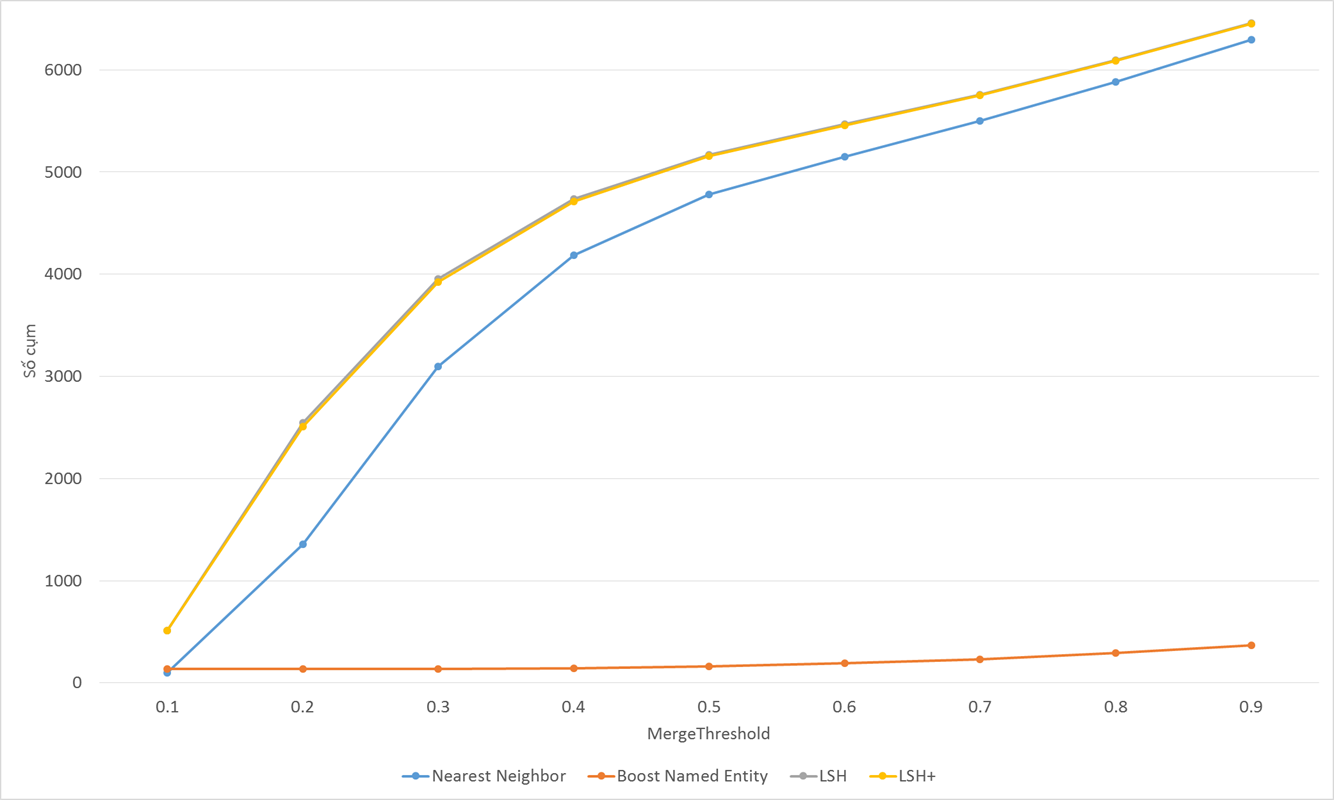
\includegraphics[width=1\linewidth]{Chapter4/Chapter4Figs/ThresholdVsClusterCount}
			\caption{Ảnh hưởng của giá trị threshold đến số cụm}
			\label{fig:thresholdvsclustercount}
		\end{sidewaysfigure}
		
		\begin{figure}
			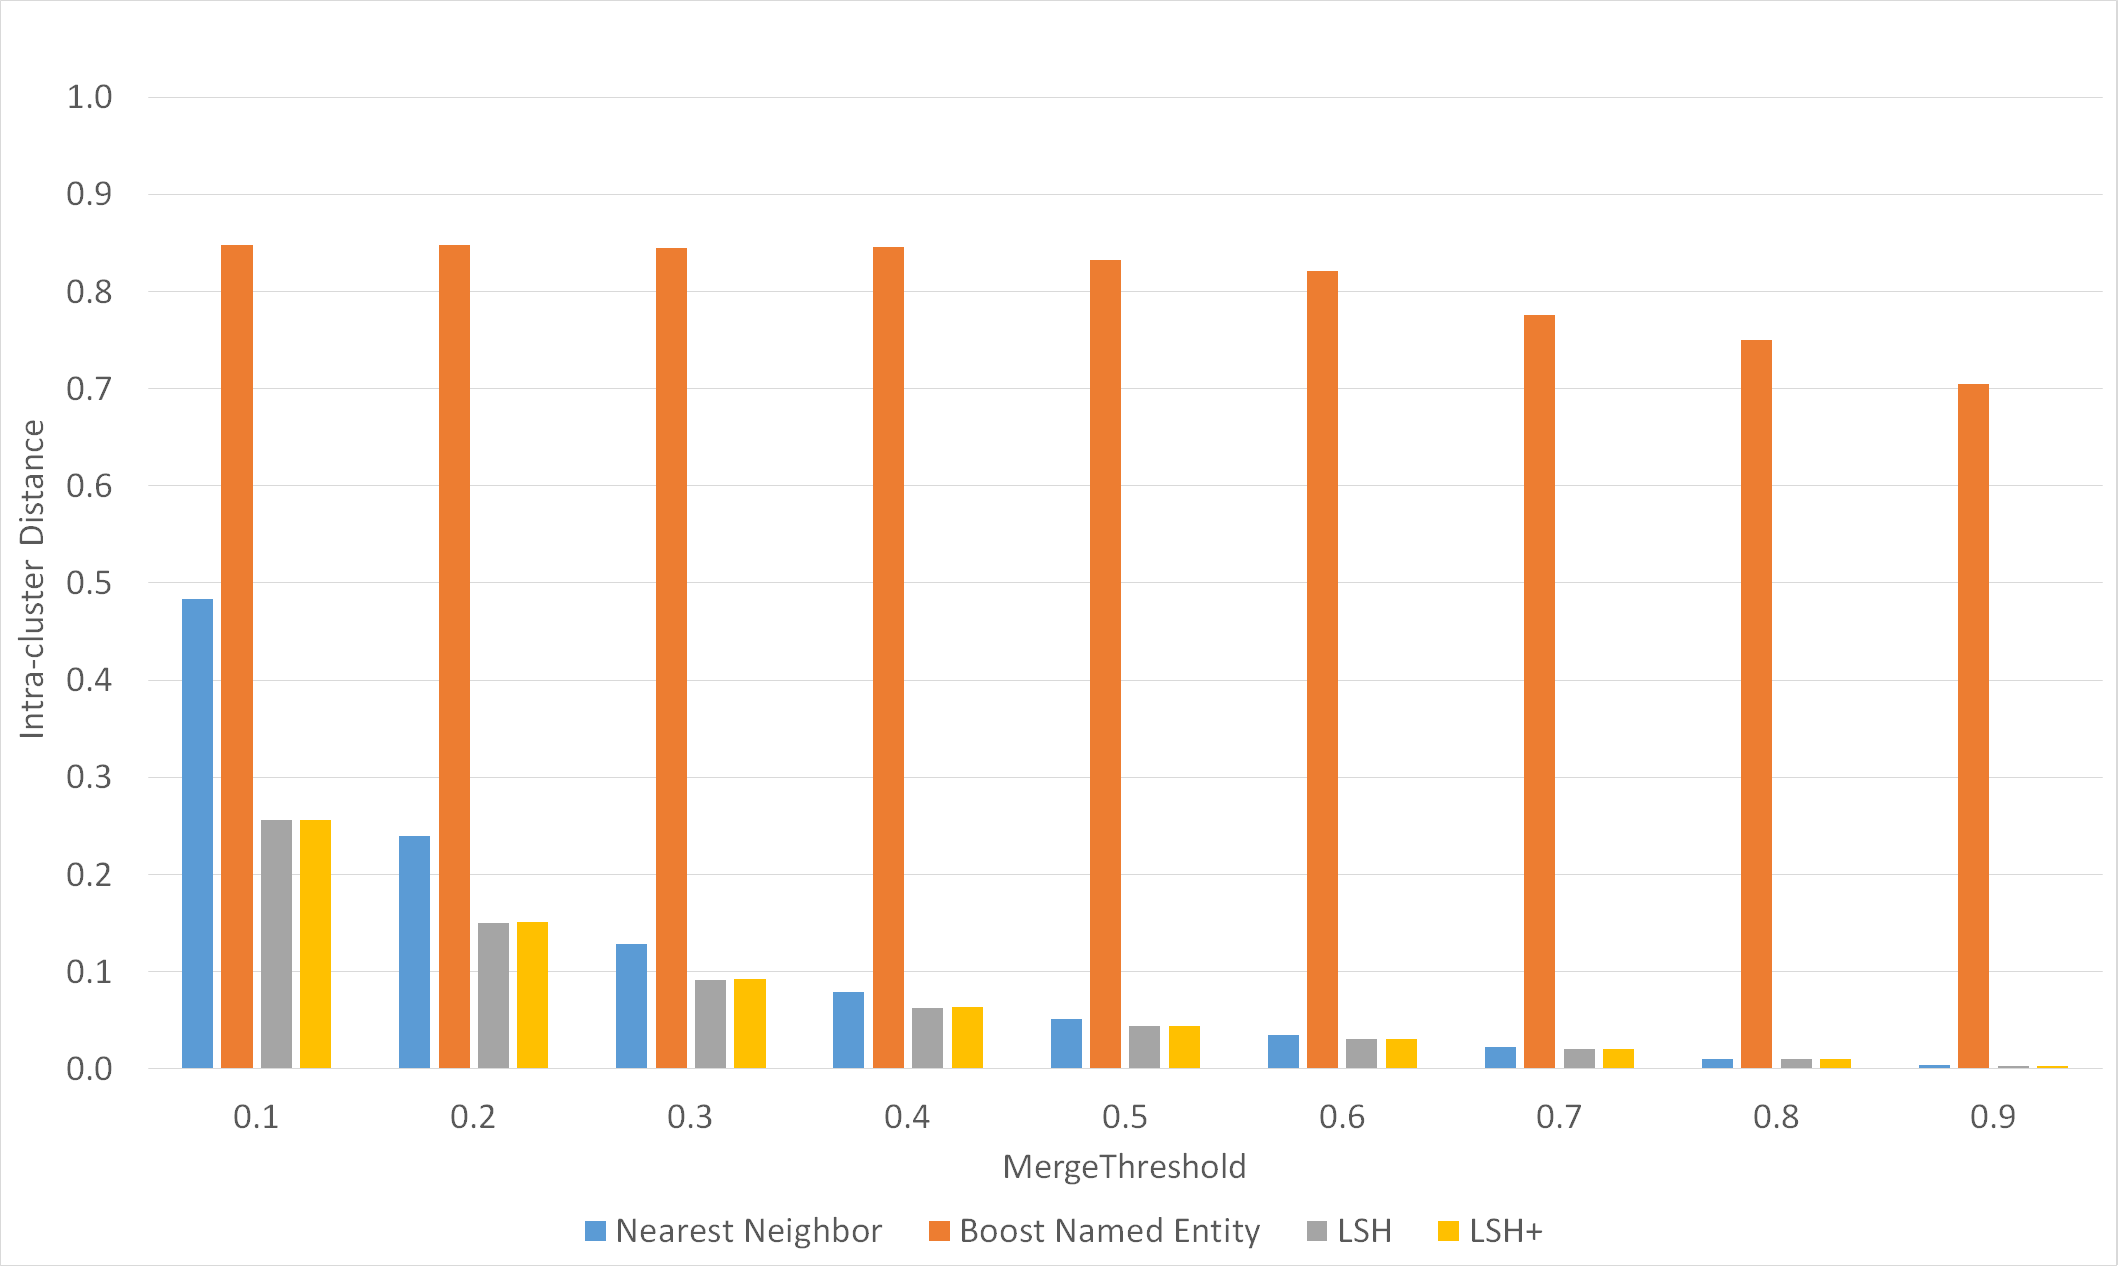
\includegraphics[width=0.9\linewidth]{Chapter4/Chapter4Figs/MergeThresholdVSIntraDistance}
			\caption{Ảnh hưởng của giá trị threshold đến intracluster distance}
			\label{fig:thresholdvslocal}
		\end{figure}
		
		\begin{figure}[H]
			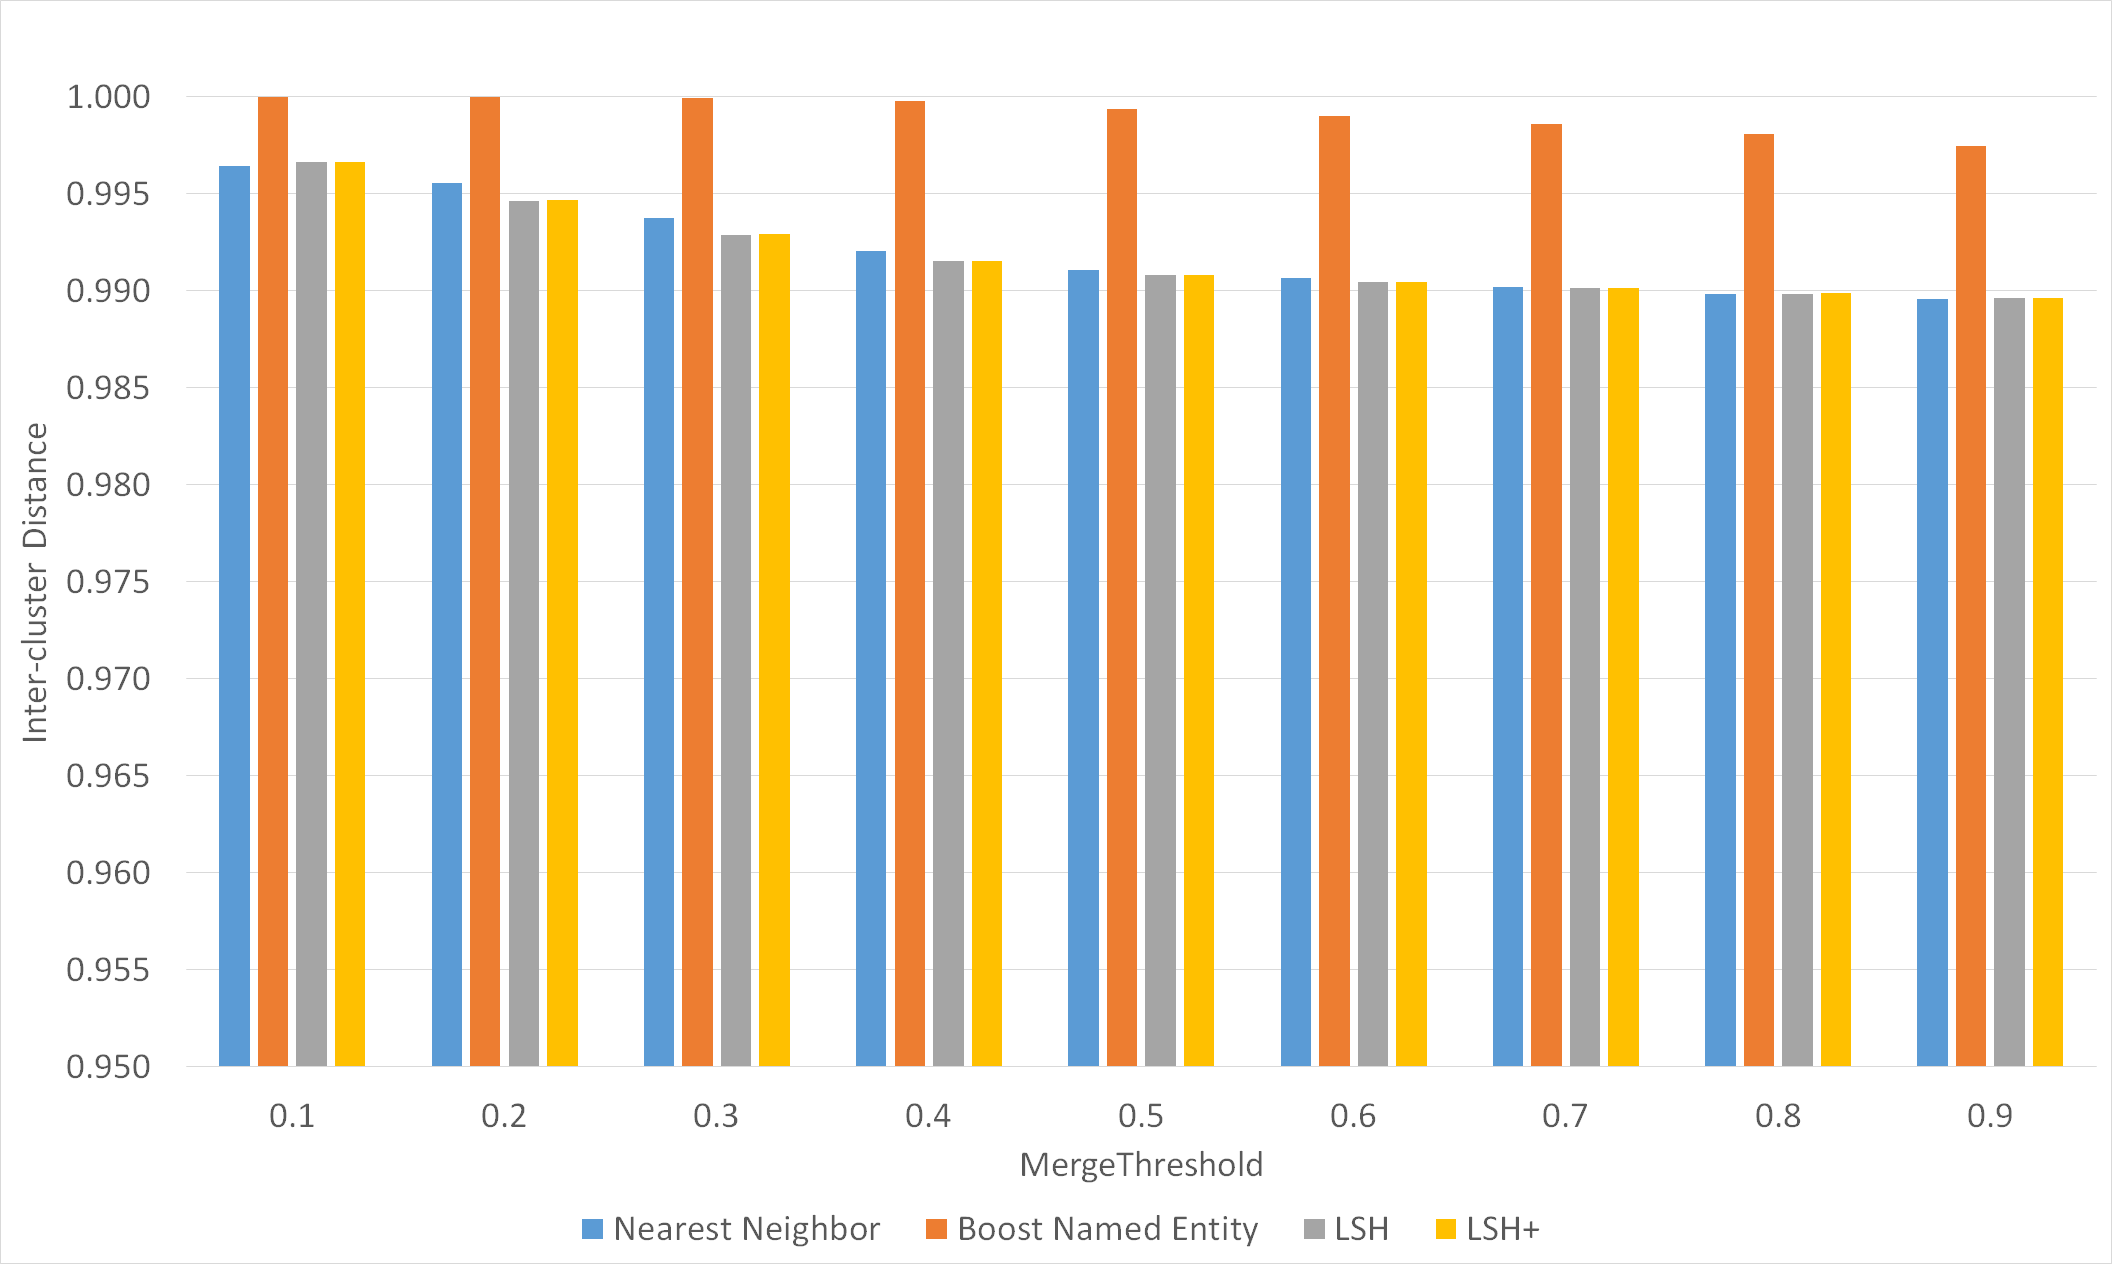
\includegraphics[width=0.9\linewidth]{Chapter4/Chapter4Figs/MergeThresholdVSInterDistance}
			\caption{Ảnh hưởng của giá trị threshold đến intercluster distance}
			\label{fig:thresholdvsglobal}
		\end{figure}
	
	Hình \ref{fig:thresholdvsruntime} cho thấy đối với cùng số lượng mẫu trong dữ liệu, hai thuật toán LSH xử lý nhanh nhất, kế đến là Nearest Neighbor và cuối cùng là thuật toán Boost Named Entity. Giá trị của MergeThreshold không có ảnh hưởng rõ rệt đến thời gian chạy của thuật toán Nearest Neighbor và LSH, tuy nhiên thuật toán Boost Named Entity thì lại tăng đáng kể. 
	
	Lý do chính thuật toán Boost Named Entity có thời gian xử lý lâu như vậy (gấp 10-600 lần các thuật toán còn lại) là vì thư viện nhận diện thực thể tiếng Việt được sử dụng có thời gian xử lý khá chậm, chiếm phần lớn thời gian thực thi của thuật toán này.
		\begin{sidewaysfigure}
			\centering
			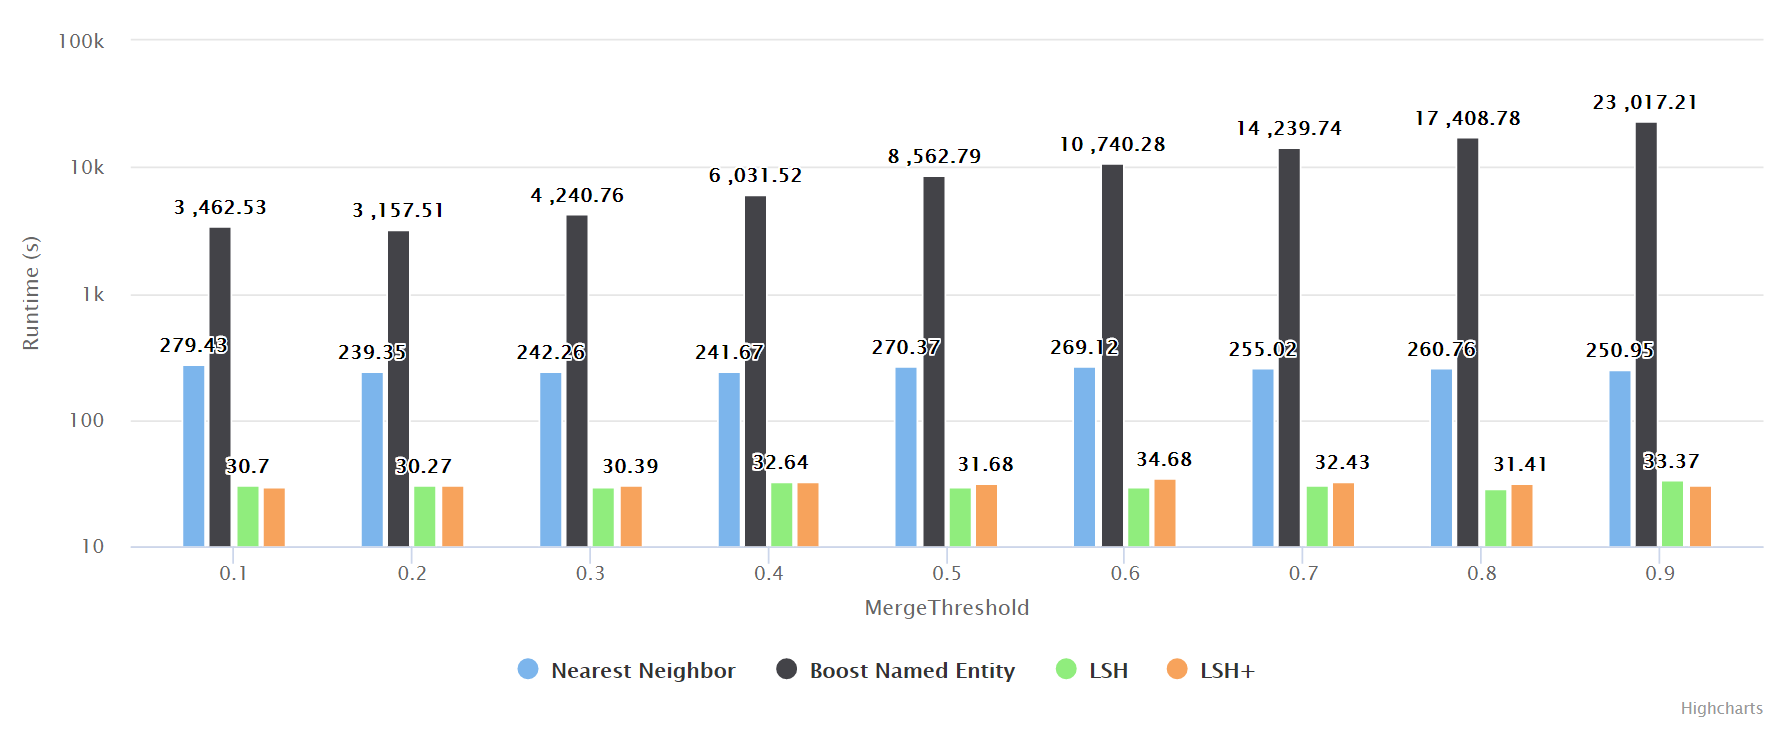
\includegraphics[width=1\linewidth]{Chapter4/Chapter4Figs/ThresholdVsRuntime}
			\caption{Ảnh hưởng của giá trị threshold đến thời gian thực thi}
			\label{fig:thresholdvsruntime}
		\end{sidewaysfigure}

	\subsection{Nhận định về các tham số của LSH}
	Thử nghiệm với thuật toán LSH cải tiến, theo Bảng \ref{tab:LSHParams} và Hình \ref{fig:lshruntime}, với giá trị MergeThreshold cố định bằng 0.5, số hash table lẫn số siêu phẳng đều tỷ lệ nghịch với số cụm thu được, tuy nhiên chúng không làm số cụm thay đổi nhiều như giá trị MergeThreshold.
	
	Về mặt thời gian xử lý, số lượng hash table tăng giảm làm thay đổi trực tiếp thời gian thực thi thuật toán. Trong khi đó, số siêu phẳng hầu như không gây ảnh hưởng nhiều.

	\begin{sidewaysfigure}
		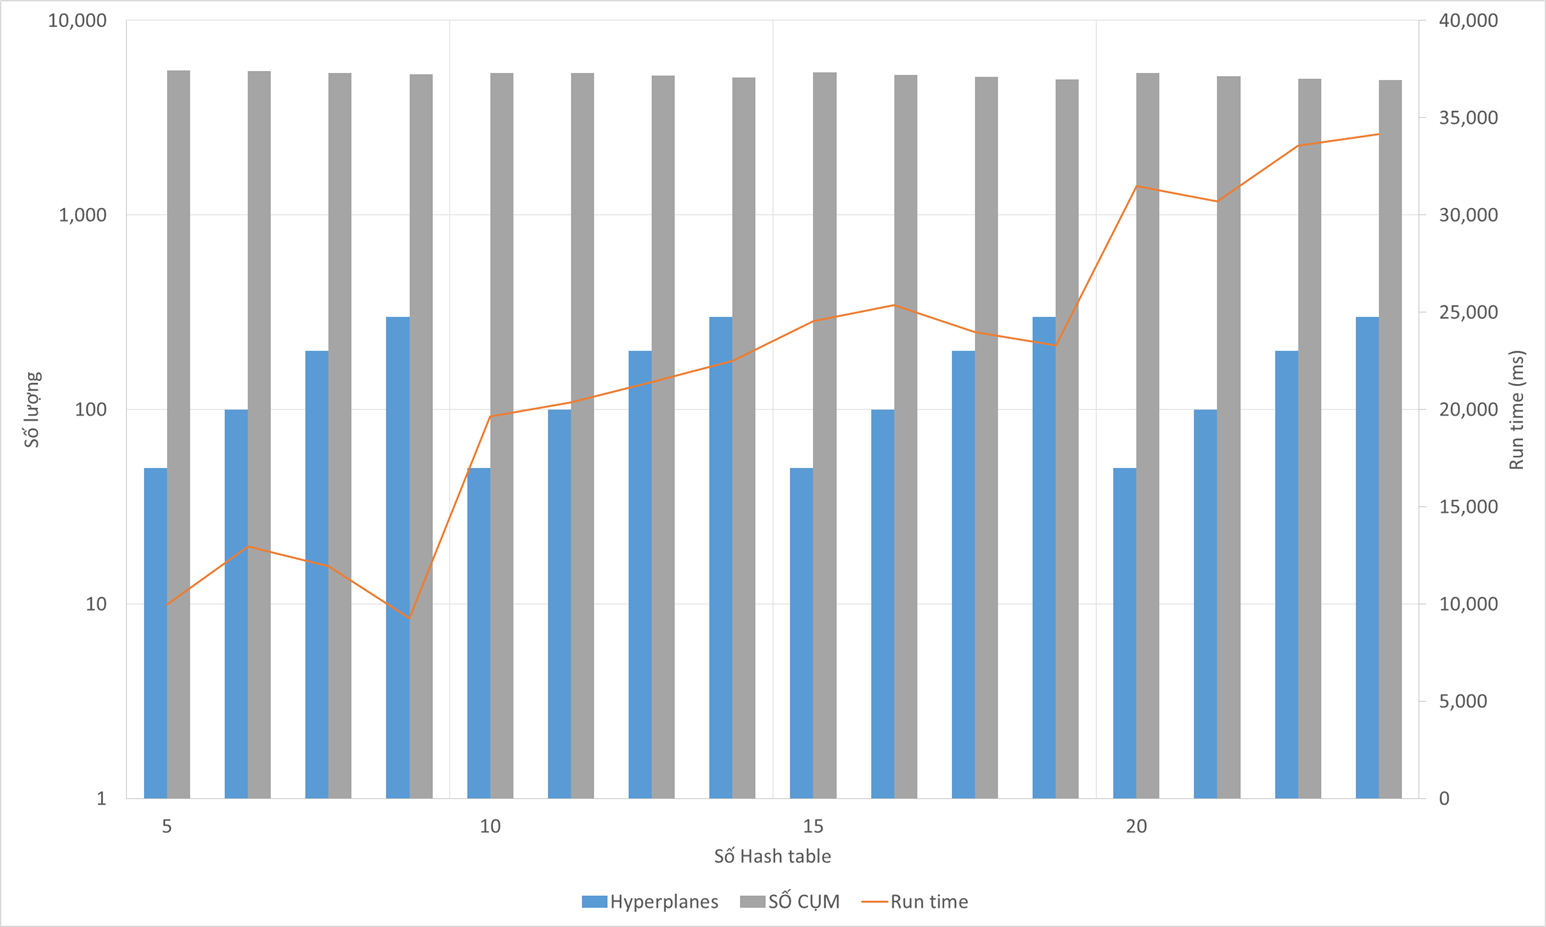
\includegraphics[width=1\linewidth]{Chapter4/Chapter4Figs/LSHRuntime}
		\caption{Ảnh hưởng của các tham số đến thời gian thực thi và số cụm của LSH}
		\label{fig:lshruntime}
	\end{sidewaysfigure}
	
\section{Kết chương}
Qua các kết quả thử nghiệm, chương này đã thể hiện được một số tính chất của các thuật toán được đánh giá như tốc độ, số lượng và chất lượng cụm kết quả. Ta thấy thuật toán LSH có tốc độ xử lý nhanh trong khi vẫn giữ được độ chính xác tốt so với thuật toán Nearest Neighbor. Riêng thuật toán Boost Named Entity do hạn chế bởi thư viện nhận diện thực thể nên thời gian thực thi lẫn chất lượng kết quả gom cụm chưa được tốt.